\chapter{Ergänzende Abbildungen}

\begin{figure}[H]
    \centering
    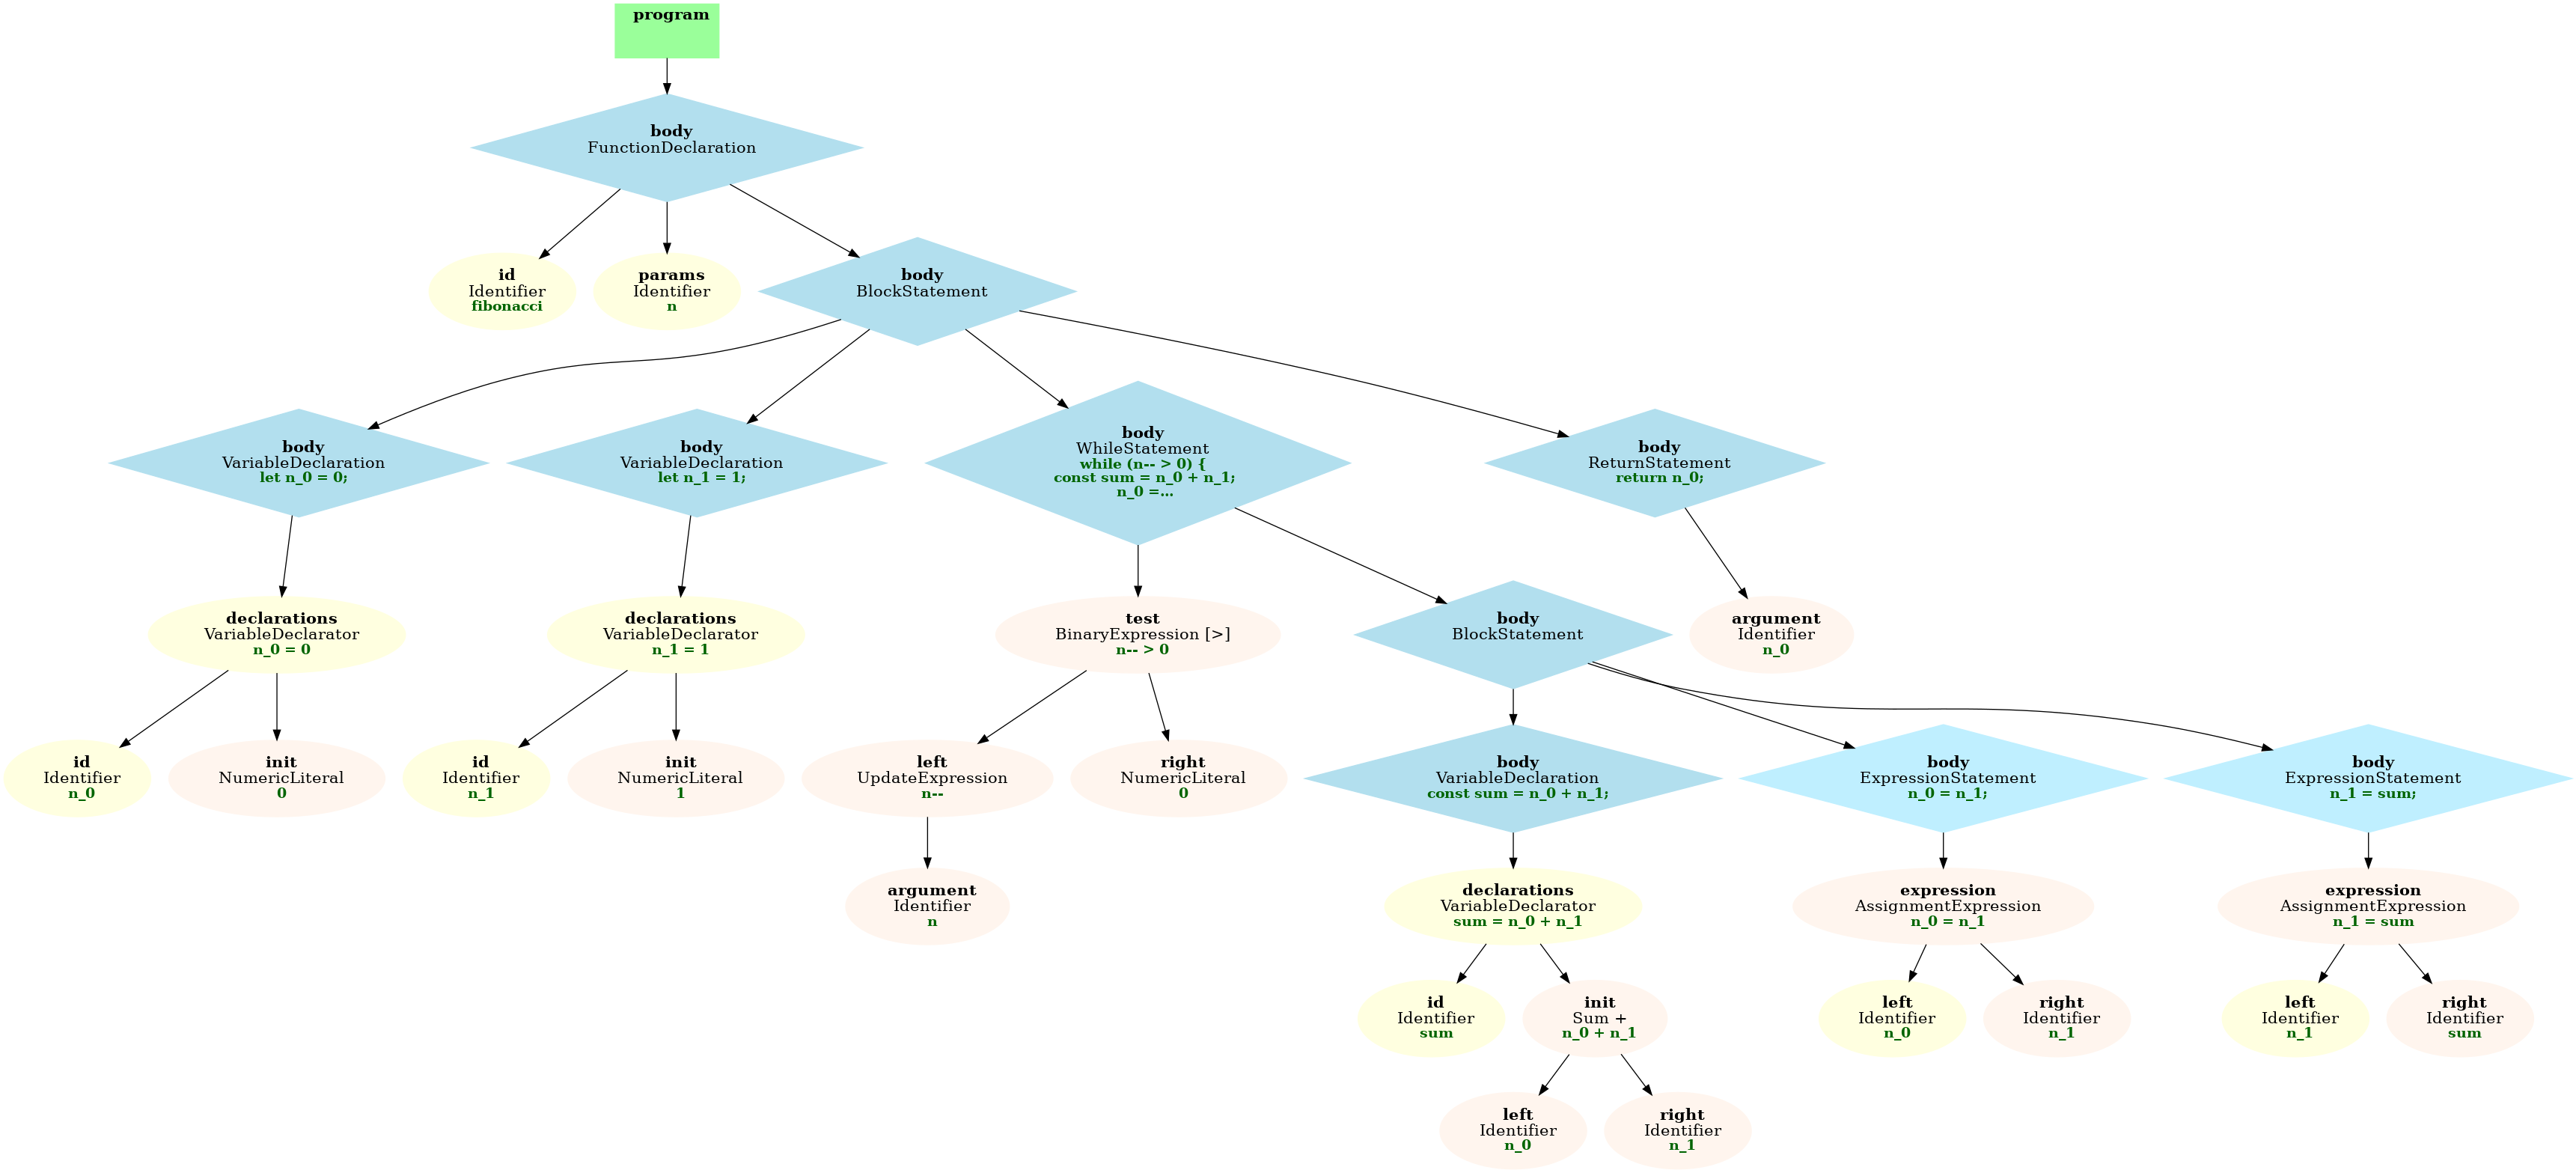
\includegraphics[width=0.95\textwidth]{./img/js-tree-fibonacci}
    \caption[Vollständiger Syntaxbaum für Fibonacci-Zahlen-Programm]{Vollständiger Syntaxbaum zum JavaScript-Programm für Fibonacci-Zahlen}
    \label{fig:JsFibonacciBaum}
\end{figure}

\begin{figure}[H]
    \centering
    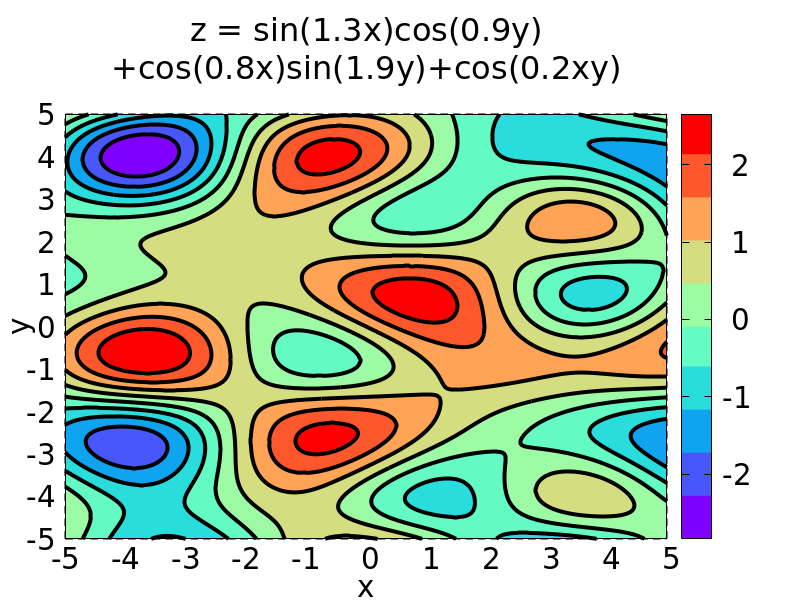
\includegraphics[width=0.95\textwidth]{./gnuplot/example-contour-field-complex}
    \caption[Konturlinien einer komplexen Funktion]{Konturlinien mit farbiger Hervorhebung für eine Funktion. Jede Farbe entspricht einem Funktionswert, wie er in der Legende rechts zu sehen ist.}
    \label{fig:ContourComplexFun}
\end{figure}

\begin{figure}[H]
    \centering
    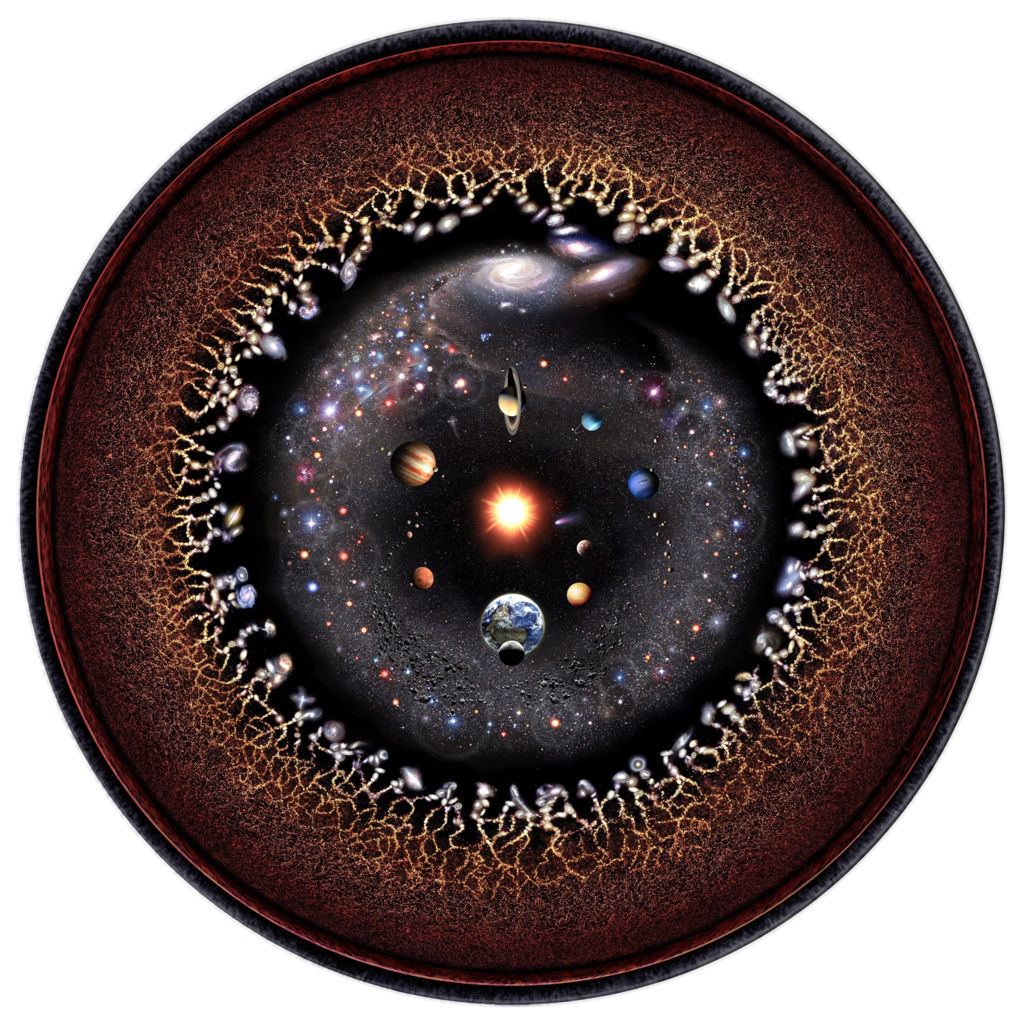
\includegraphics[width=0.95\textwidth]{./img/universe-log-scale}
    \caption[Künstlerische Darstellung des beobachtbaren Universums in logarithmischer Skalierung]{Künstlerische Darstellung des beobachtbaren Universums in logarithmischer Skalierung und Zentrierung auf das Sonnensystem. Abgebildet sind die inneren und äußeren Planeten des Sonnensystems, der Kuipergürtel, die Oortsche Wolke, Alpha Centauri, Perseusarm, die Milchstraße, der Andromedanebel, Nachbargalaxien, das Kosmische Netz, die Kosmische Hintergrundstrahlung und der Plasmazustand kurz nach dem Urknall. Quelle: \href{https://commons.wikimedia.org/wiki/User:Unmismoobjetivo}{Pablo Carlos Budassi}, \href{https://commons.wikimedia.org/wiki/File:Observable_universe_logarithmic_illustration.png}{wikimedia}}
    \label{fig:UniLogScale}
\end{figure}

\begin{figure}[H]
    \centering
    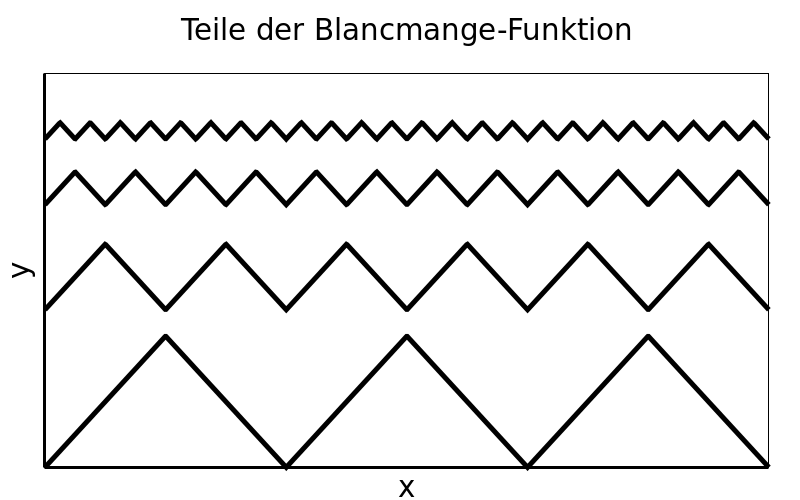
\includegraphics[width=0.55\textwidth]{./gnuplot/blancmange-function-parts}
    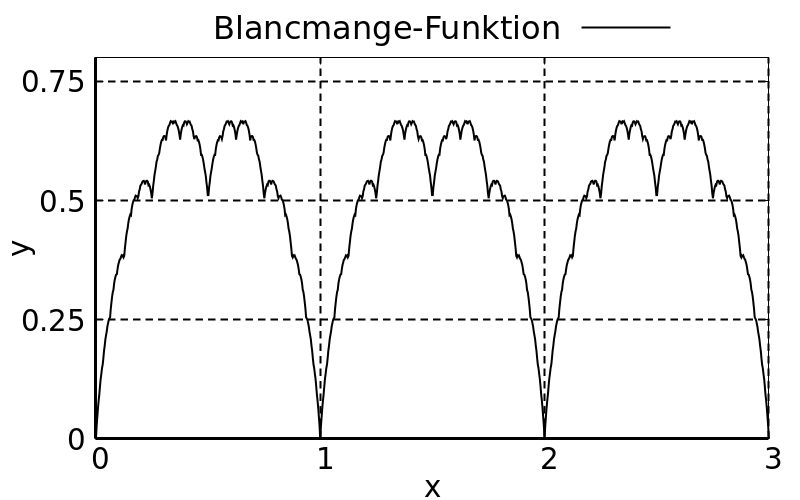
\includegraphics[width=0.45\textwidth]{./gnuplot/blancmange-function-total}
    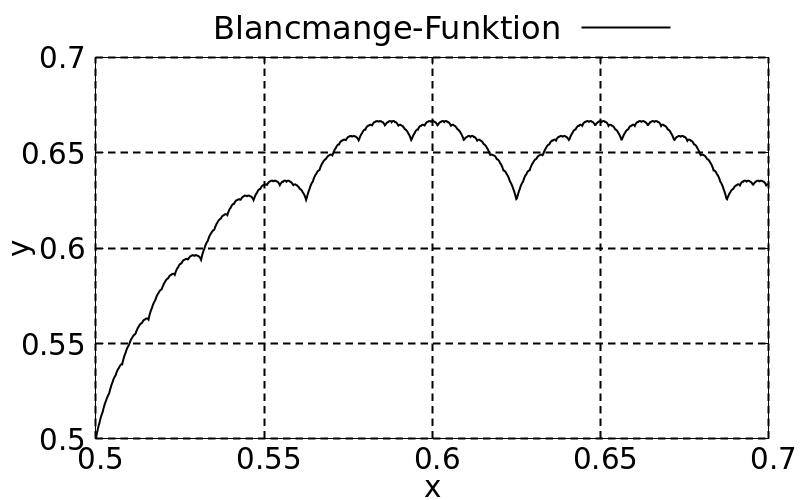
\includegraphics[width=0.45\textwidth]{./gnuplot/blancmange-function-zoomed}
    \caption[Konstruktion der Blancmange-Funktion]{Die Blancmange-Funktion, welche sich durch Addition von Dreiecksschwingungen ergibt. Sie ist zwar überall stetig, aber nirgends differenzierbar. Egal, wie stark man einen Ausschnitt der Kurve vergößert, die Zackenstruktur bleibt bestehen und lässt sich nicht durch eine Gerade annähern.}
    \label{fig:BlancmangeFunction}
\end{figure}

\begin{figure}[H]
    \centering
    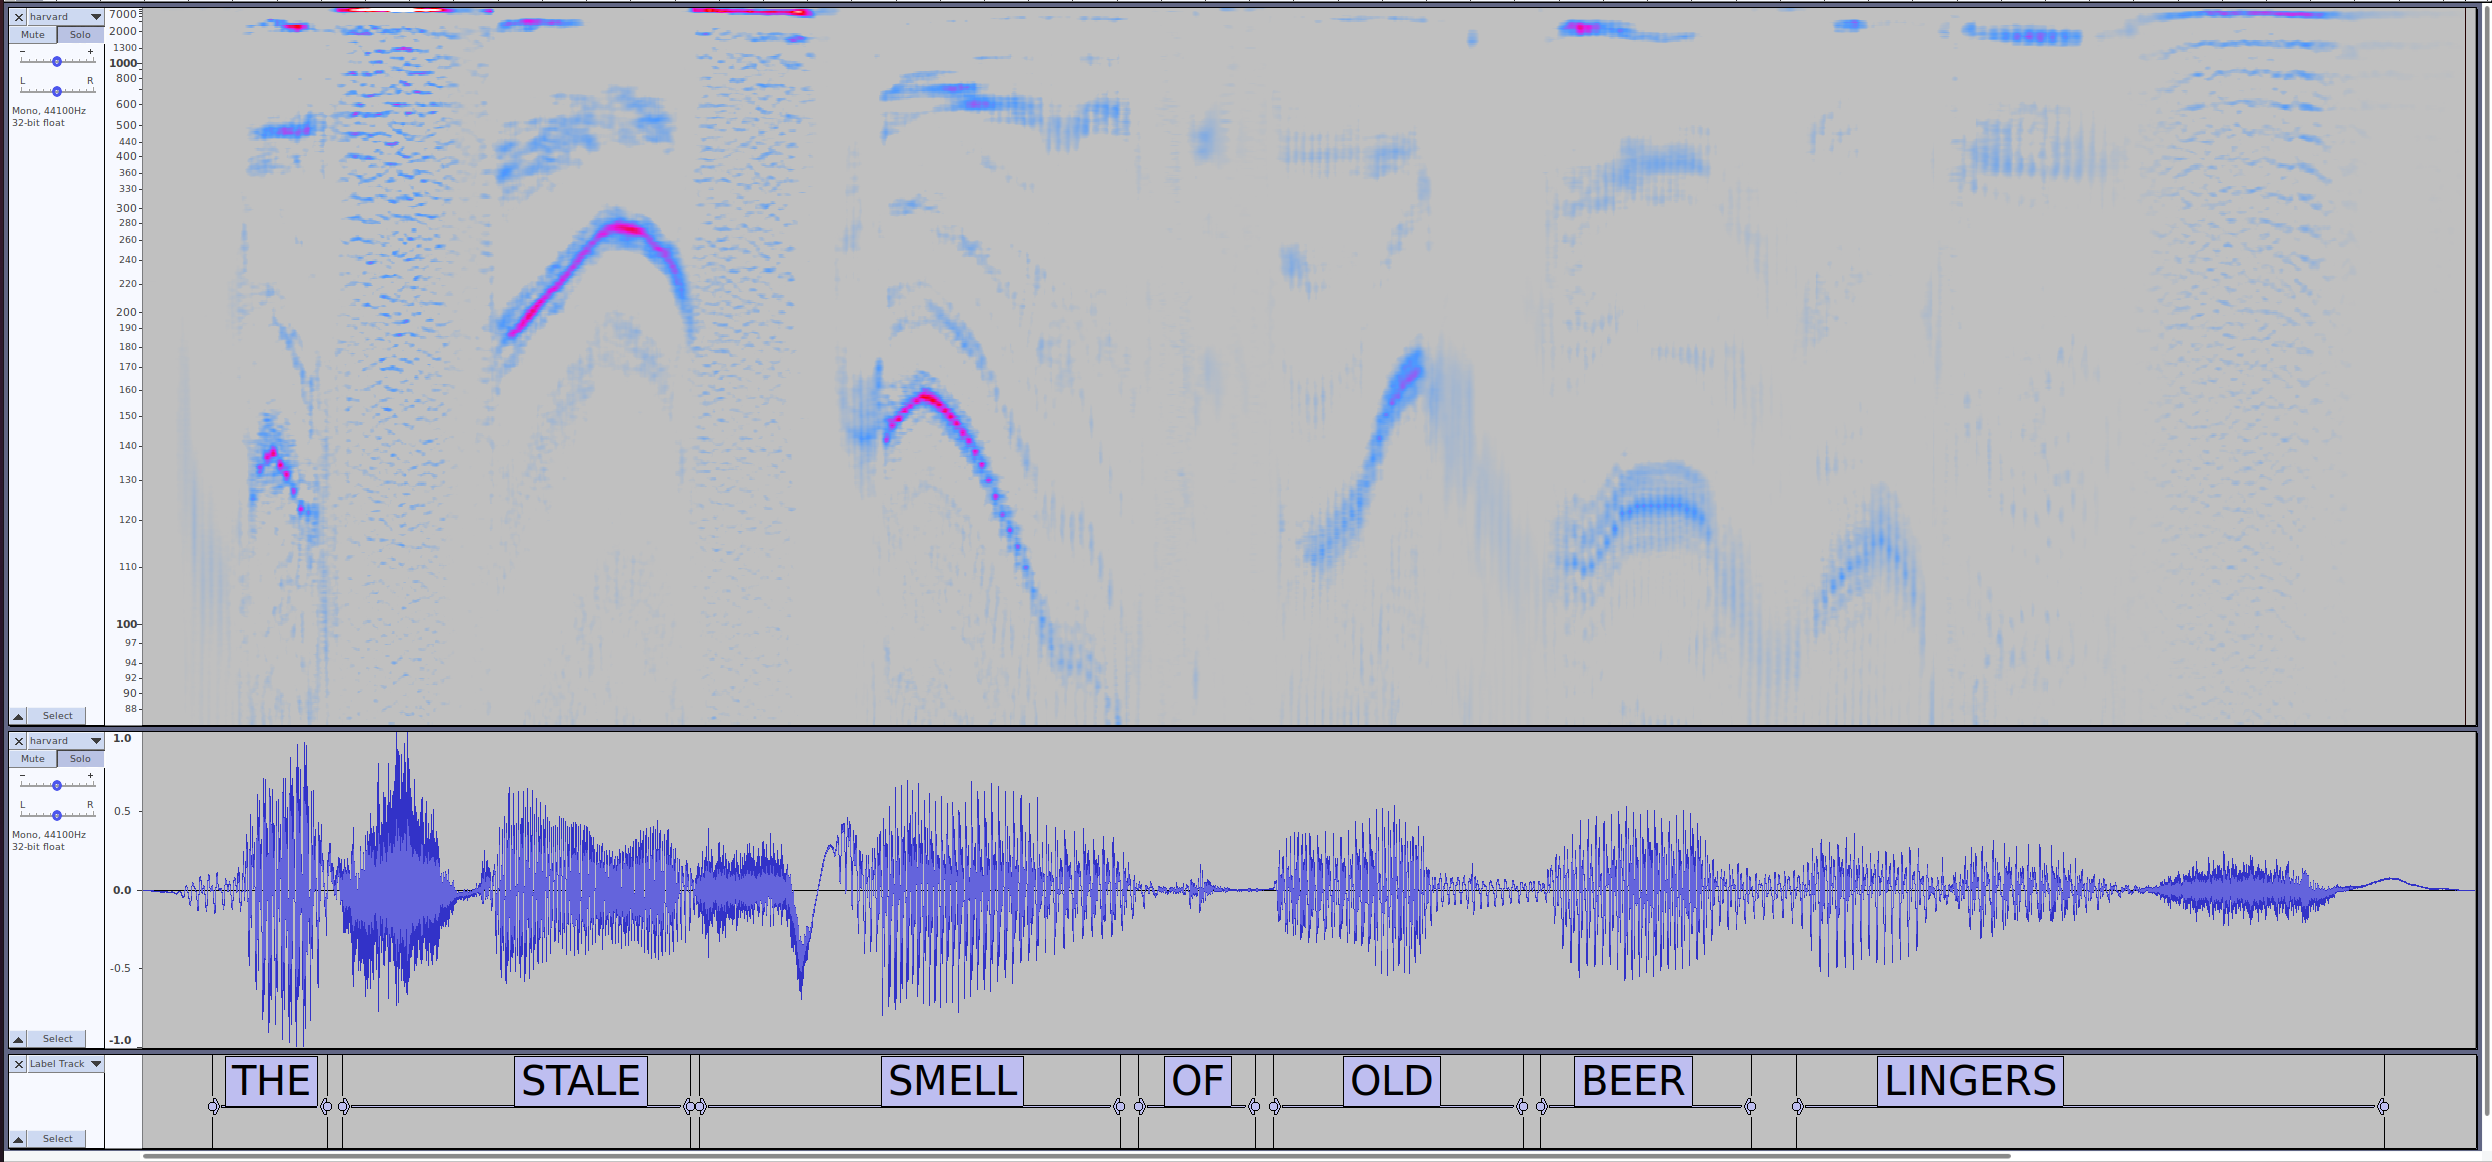
\includegraphics[width=0.95\textwidth]{./img/speech-recognition}
    \caption[Frequenzspektrum eines Audiosignals]{Graphische Darstellung des Audiosignals des gesprochenen Satzes "The stale smell of old beer lingers". Oben: Signal in Frequenzdomäne. Unten: Signal in Zeitdomäne. Während man im Frequenzbereich eindeutige Muster erkennt -- beispielsweise besteht der "S"-Zischlaut aus vielen Frequenzen mit etwa gleicher Amplitude -- ist es im Zeitbereich nur schwer bis gar nicht möglich, Laute oder Wörter zu erkennen.}
    \label{fig:SpeechFreq}
\end{figure}

\begin{listing}
\begin{jscode}
// @ts-check

/**
 * @typedef {{
 *   mass: number,
 *   springConstant: number,
 *   deltaTime: number,
 *   startTime:  number,
 *   endTime: number,
 *   initialPosition: number,
 *   initialVelocity: number,
 * }} PendulumConfig
 */
undefined;

/**
 * @typedef {{
 *   position: number,
 *   velocity: number,
 *   time: number,
 * }} PendulumDataPoint
 */
undefined;

/**
 * @param {PendulumConfig} config
 * @return {PendulumDataPoint[]}
 */
function simulatePendulum(config) {
    /** @type {PendulumDataPoint[]} */
    const result = [{
        position: config.initialPosition,
        velocity: config.initialVelocity,
        time: config.startTime,
    }];
    for (let t = config.startTime; t <= config.endTime; t += config.deltaTime) {
        const x = result[result.length - 1].position;
        const v = result[result.length - 1].velocity;
        const newX = x + config.deltaTime * v;
        const newV = v - config.deltaTime * config.springConstant / config.mass * x
        result.push({
            position: newX,
            velocity: newV,
            time: t + config.deltaTime,
        });
    }
    return result;
}
\end{jscode}
    \caption[Code Nummerische Lösung DGL]{Auszug des JavaScript-Programms zur nummerischen Lösung der Differentialgleichung für die harmonische Schwingung. Dargestellt ist die Funktion, welcher iterativ Position und Geschwindigkeit zum nächsten Zeitpunkt berechnet.}
    \label{lst:NumSolveCode}
\end{listing}